% %%%%%%%%%%%%%%%%%%%%%%%%%%%%%%%%%%%%%%%%%%%%%%%%%%%%%%%%%
% | - Electrochemical OER Application
% %%%%%%%%%%%%%%%%%%%%%%%%%%%%%%%%%%%%%%%%%%%%%%%%%%%%%%%%%
%
% __|
% %%%%%%%%%%%%%%%%%%%%%%%%%%%%%%%%%%%%%%%%%%%%%%%%%%%%%%%%%



% %%%%%%%%%%%%%%%%%%%%%%%%%%%%%%%%%%%%%%%%%%%%%%%%%%%%%%%%%
% | - Short Intro EChem Section
%
% __|
% %%%%%%%%%%%%%%%%%%%%%%%%%%%%%%%%%%%%%%%%%%%%%%%%%%%%%%%%%
% | - PARAGRAPH BODY
%
% TODO In the previous sections make sure to highlight the alpha and rutile IrO3 phases explicitly so that this sentence makes sense here.
We next performed \latin{ab-initio} thermodynamic simulations to elucidate the electrochemical operational stability of \IrOx and the oxygen evolution reaction (OER) activity of various \IrOthree phases previously computed.
%
In particular, we compare the stability and activity of the most stable \IrOtwo and \IrOthree polymorphs
(namely \rIrOtwo and our newly discovered \aIrOthree),
and the \rIrOthree polymorph.
%
In addition, we computed the OER activity of a delithiated form of a recently reported $\beta$-Li\textsubscript{x}IrO\textsubscript{3} structure
(referred to here as \bIrOthree),
as it is a notable example of a well characterized experimental \IrOthree OER catalyst with exceptional activity.
\cite{Pearce2017,Pearce2019}
%
The OER activity was computed assuming the associative OER mechanism and utilizing the limiting potential analysis and computational hydrogen electrode (see Supporting Information).
\cite{Man2011,Rossmeisl2007,Kitchin2004}
% __|
% %%%%%%%%%%%%%%%%%%%%%%%%%%%%%%%%%%%%%%%%%%%%%%%%%%%%%%%%%


% %%%%%%%%%%%%%%%%%%%%%%%%%%%%%%%%%%%%%%%%%%%%%%%%%%%%%%%%%
% | - Bulk Pourbaix Diagram
%
% Explain the Ir and IrO[4-] species
% QUESTION Use E or U for potential variable
% __|
% %%%%%%%%%%%%%%%%%%%%%%%%%%%%%%%%%%%%%%%%%%%%%%%%%%%%%%%%%
% | - PARAGRAPH BODY
%
The bulk Pourbaix diagram of the Ir-H\textsubscript{2}O system is shown in Figure~\ref{fig:bulk_pourbaix}.
%
The diagram was constructed by considering the equilibrium between the following species: Ir, \rIrOtwo, \aIrOthree, \rIrOthree, \bIrOthree, and an aqueous dissolved \ce{IrO^{4-}} species.
%
We utilized a free energy correction scheme to reproduce the experimental free energy of \IrOtwo relative to the \ce{Ir} reference state
(see the Supporting Information for further details).
%
While Ir and \rIrOtwo are most stable at low bias, \aIrOthree becomes the thermodynamically dominant phase under the relevant conditions for the OER (potentials around \mytilde1.23 \VRHE and an acidic environment)
%
% I want to be careful about how I talk about the metastable structures in the bulk Pourbaix, they strictly speaking shouldn't be there at all
The stability regions of the metastable \rIrOthree and \bIrOthree phases (In the absence of any other \IrOthree polymorph) are indicated by unfilled solid lines, and show that these phases also have a large stability window relative to \IrOtwo and the Ir ion.
%
There are twenty-one unique \IrOthree polymorphs discovered in our search which have a region of stability in the bulk Pourbaix plot, in the pH window of zero to sixteen.
%
% TODO Create energy table for main bulk systems in SI
% The similar formation energies (see Table \ref{table:oer_table}) for all three \IrOthree species suggest some or all of these \IrOthree phases may be present and are stable under OER conditions.
% __|
% %%%%%%%%%%%%%%%%%%%%%%%%%%%%%%%%%%%%%%%%%%%%%%%%%%%%%%%%%


% =========================================================
% FIGURE ==================================================
% =========================================================
% | - Figure | Bulk Pourbaix Diagram
\begin{figure*}[!htb]
\centering
\makebox[\textwidth][c]{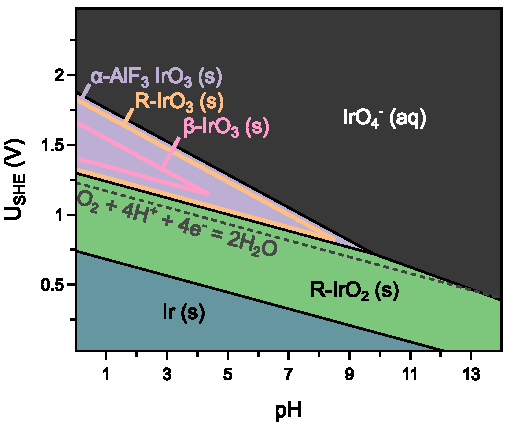
\includegraphics
{02_figures/oer_activity_stability/00_master__bulk-pourbaix__v6.pdf}}
\caption{\label{fig:bulk_pourbaix}
%
Revised bulk Pourbaix diagram of the \ce{Ir}-\ce{H2O} system as a function of applied potential and pH.
%
The diagram was constructed with Ir(s) (blue), \rIrOtwo (green), various \IrOthree polymorphs and a dissolved \ce{IrO^{4-}} ion species (dark grey).
%
The stability regions corresponding to the metastable \rIrOthree and \bIrOthree polymorphs, in the absence of any competing \IrOthree phase, are displayed as yellow and pink lines, respectively.
%
The thermodynamic onset of OER (water equilibrium at \num{1.23} \VRHE) is also shown.
%
% The most stable system studied (see Table XX in SI for a full list) are Ir-metal Ir(s) (blue), a \rIrOtwo (green), and a dissolved \ce{IrO4[4-]} (grey).
%
% These are compared to the \ce{IrO_3} polymorphs, \aIrOthree (purple), \rIrOthree (orange), and \bIrOthree (pink).
}
\end{figure*}
% __| =====================================================
% =========================================================


% %%%%%%%%%%%%%%%%%%%%%%%%%%%%%%%%%%%%%%%%%%%%%%%%%%%%%%%%%
% | - Introduction to OER Results
%
% __|
% %%%%%%%%%%%%%%%%%%%%%%%%%%%%%%%%%%%%%%%%%%%%%%%%%%%%%%%%%
% | - PARAGRAPH BODY
%
The results of the electrochemical activity and surface stability analysis are summarized in Figure~\ref{fig:oer_volcano}.
%
There, we report the surface energy Pourbaix plots and OER activity for various surface facets at select coverages (*OH, *O, and bare) of the four \IrOx polymorphs from Figure \ref{fig:bulk_pourbaix}.
%
The surface stability Pourbaix plots inform which surface facets and surface coverage species are thermodynamically preferred under OER conditions.
%
This analysis allows us to consider both stability and activity of OER active sites and their surfaces.
%
For each polymorph, surfaces were constructed by cleaving along high symmetry facet planes.
% __|
% %%%%%%%%%%%%%%%%%%%%%%%%%%%%%%%%%%%%%%%%%%%%%%%%%%%%%%%%%


% %%%%%%%%%%%%%%%%%%%%%%%%%%%%%%%%%%%%%%%%%%%%%%%%%%%%%%%%%
% | - Surface Energy Pourbaix Analysis
%
% __|
% %%%%%%%%%%%%%%%%%%%%%%%%%%%%%%%%%%%%%%%%%%%%%%%%%%%%%%%%%
% | - PARAGRAPH BODY
%
Figure~\ref{fig:oer_volcano}a reports the surface energy Pourbaix plots as a function of applied potential (at pH\num{=0}) for the four \IrOx crystals of interest.
%
For each facet we computed the surface free energy for three coverages, bare, *OH, and *O.
%
At modest overpotentials ($\eta$ \mytilde\num{0.3} or equivalently potentials of \mytilde\num{1.5} \VRHE) the convex hull is populated solely by oxygen terminated surfaces.
%
% COMBAK, Revise "mainly" if we include some different coverages
Consequently, we consider mainly oxygen terminated surfaces for the OER analysis.
%
These results are comparable to previous studies on the electrochemical stability of \IrOtwo surfaces~\cite{Nattino2019},
but without considering highly reconstructed facets such as (101).
% __|
% %%%%%%%%%%%%%%%%%%%%%%%%%%%%%%%%%%%%%%%%%%%%%%%%%%%%%%%%%


% =========================================================
% FIGURE ==================================================
% =========================================================
% | - Figure | OER Volcano/Surface Pourbaix
\begin{figure*}
\centering
\makebox[\textwidth][c]{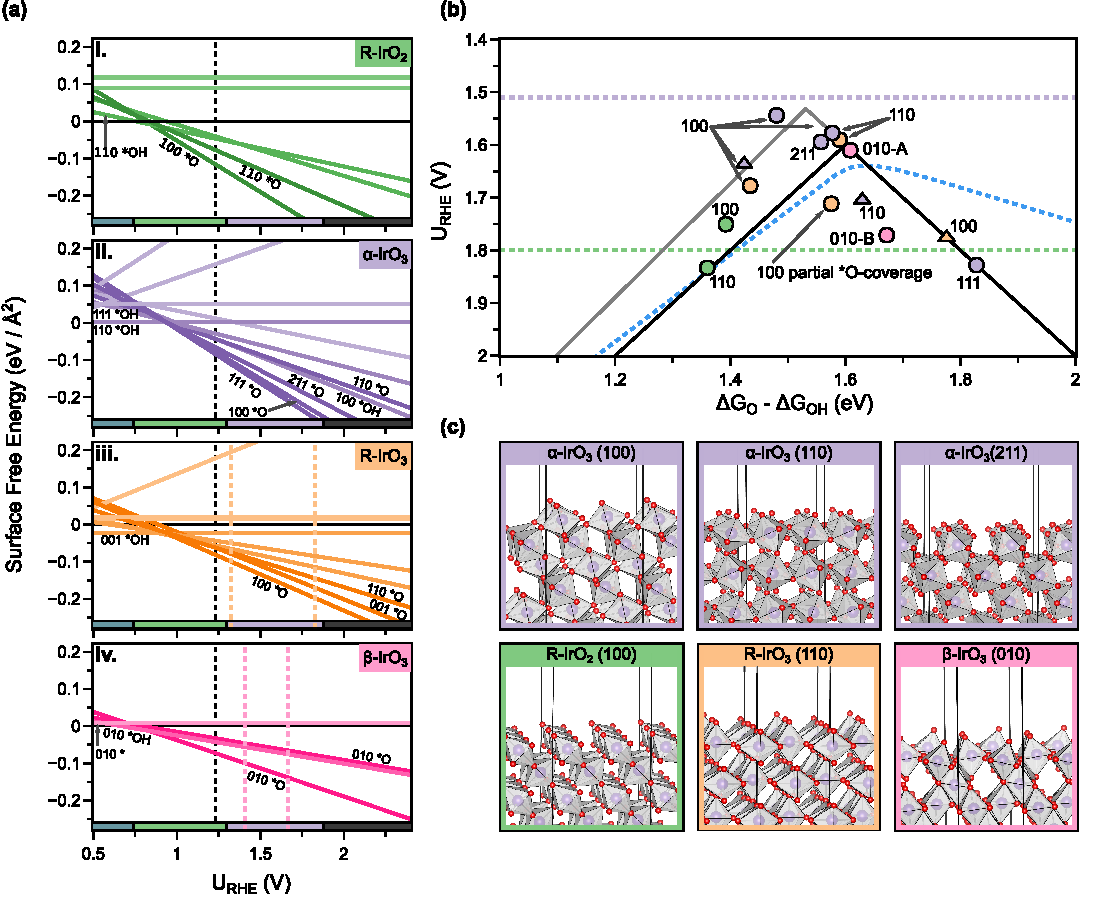
\includegraphics
{02_figures/oer_activity_stability/00_oer_plot_v10__downsampled_0900x0900.pdf}}
\caption{\label{fig:oer_volcano}
% TODO Insert green band into figure, insert experimental references for this
%
Summary of OER results for the following four bulk structures of \IrOx: \rIrOtwo (green), \aIrOthree (purple), \rIrOthree (orange), and \bIrOthree (pink).
%
(a) Surface energy Pourbaix diagrams for each structure, with the surface energy of various facets and coverages shown as a function of applied potential (\VRHE).
%
Surfaces with coverages of bare surfaces (light lines), *OH covered surfaces (medium lines) and *O terminated surfaces (thick lines) are shown.
%
The bulk Pourbaix diagram's bounds of stability at pH \num{0} are superimposed at the bottom of each subplot.
%
The pseudo-stability regimes for the meta-stable \bIrOthree and \rIrOthree are indicated by dashed vertical lines.
%
(b) OER activity volcano for \IrOx systems considered utilizing the \DGOmOH thermochemical descriptor.
%
% TODO Add citations here
The horizontal lines correspond to recent experimental OER limiting potentials for \IrOtwo and \IrOthree~\cite{Seitz2016}, and were taken at a current density of \SI[mode=text]{10}{\mA\per\cm\squared}.
% The purple dotted line corresponds to the experimental limiting potential at \num{10} mA cm\textsuperscript{-2} for \ce{IrO_3} \cite{Seitz2016},
% while the green band corresponds to the range of experimentally observed overpotentials for pristine \ce{IrO_2} catalysts as reported in literature.
%
(c) Corresponding structural models for select OER surfaces.
%
% (c) Select surface facets for the four \IrOx crystal systems considered.
%
Color legend: oxygen (red), purple (iridium), coordination motif (white).
}
\end{figure*}
% __| =====================================================
% =========================================================


% %%%%%%%%%%%%%%%%%%%%%%%%%%%%%%%%%%%%%%%%%%%%%%%%%%%%%%%%%
% | - OER Volcano
% TODO We don't mention new old/new scaling volcanos
% __|
% %%%%%%%%%%%%%%%%%%%%%%%%%%%%%%%%%%%%%%%%%%%%%%%%%%%%%%%%%
% | - PARAGRAPH BODY
%
% Replace G_O and G_OH with my custom macros for consistency
The OER activity (in terms of the limiting potential) for select oxygen terminated surfaces are shown in Figure \ref{fig:oer_volcano}b plotted against the \DGOmOH thermodynamic descriptor.
%
We display both thermodynamic limiting potential volcanos
(one assuming universal scaling relations and the other constructed from our fitted scaling lines)
and the kinetic OER volcano from Dickens \latin{et al.}~\cite{Dickens2019},
which tracks the required potential to reach \SI[mode=text]{10}{\mA\per\cm\squared} for a detailed microkinetic model of the OER associative pathway.
%
The thermodynamic and kinetic volcanos agree remarkably well in the strong binding leg of the volcano and all three volcano plots exhibit optimal \DGOmOH descriptor values within \num{0.1} eV/atom.
%
The corresponding surface structures for select systems are visualized in Figure \ref{fig:oer_volcano}c.
%
The \rIrOtwo surfaces bind the OER intermediates relatively strongly,
with theoretical limiting potentials of \mytilde\num{1.8} \VRHE (overpotential of \num{0.57} \VRHE) with a *O to *OOH potential limiting step.
%
% Cite Cr-IrO2 paper (ours) and something else here
These results are in agreement with previous experimental, and the latest theoretical studies.
%
The predicted overpotentials of our \rIrOtwo systems are within the range of experimentally observed overpotentials found in literature.
%
% Reference all experimental IrO2 overpotentials I can find
The surfaces of the three \IrOthree polymorphs have \DGOmOH descriptor values shifted to higher energies, indicative of weaker binding energetics (see Figure \ref{fig:scaling_relations}).
% The three \IrOthree polymorph surfaces all have a $\Delta G_\mathrm{O} - \Delta G_\mathrm{OH}$ descriptor towards the top and right of the volcano, indicative of weaker binding energetics.
%
% COMBAK Report just *OH, I have the other ones to
% O: 1.2 eV; *OOH: 1.4 eV
On average, the binding for *OH is weakened by 0.7 eV relative to \IrOtwo.
%
The highest performing systems include the (100), (110), and (211) facets of \aIrOthree, \bIrOthree (101), and \rIrOthree (110).
%
These surfaces have overpotentials of \mytilde\num{0.4} \VRHE,
which represents a \mytilde\num{0.2} \VRHE improvement over \rIrOtwo.
%
The primary driver for the improved OER activity is the higher oxidation state of \IrOthree compared to \IrOtwo
(\ce{Ir^{6+}} and \ce{Ir^{4+}}, respectively)
%
The more oxygen saturated \IrOthree systems thus bind OER intermediates more weakly, which for overbinding materials like \IrOtwo and \RhOtwo leads to more ideal scaling.
%
These results are consistent with Back \latin{et al.}, who recently demonstrated elevated activity in highly oxidized \IrOthree catalysts.\cite{Back2019}
%
The exact improvement in the theoretical overpotential is slightly dependent on the DFT level of theory and the inclusion of spin polarization, and has been discussed recently.~\cite{Seitz2016,Strickler2019}
% __|
% %%%%%%%%%%%%%%%%%%%%%%%%%%%%%%%%%%%%%%%%%%%%%%%%%%%%%%%%%
